\section{\MBSim - Program Overview}
\MBSim{} is written in the object-orientated programming language C++. 

Fig.~\ref{fig:objects} shows a class diagram.
\begin{figure}
	\centering
  	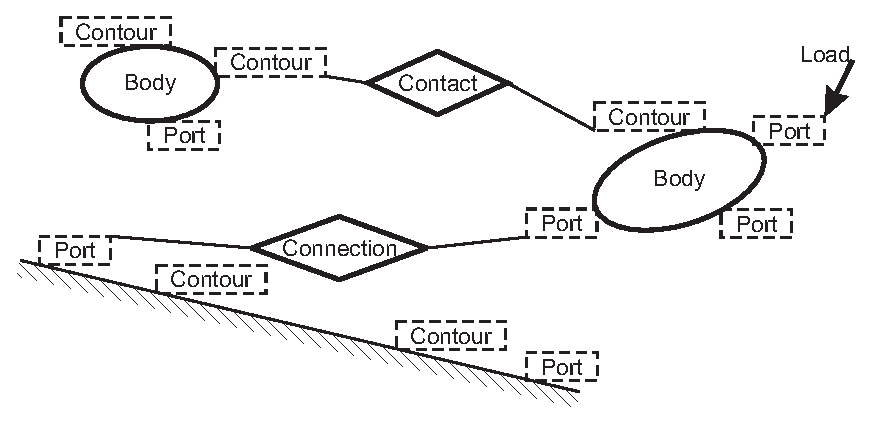
\includegraphics[width=12cm]{Figures/objectorientationMBSim.eps} % TODO
  	\caption{object structure in \MBSim}
  	\label{fig:objects}
\end{figure}
Exemplary this is a dynamical system with environment and two bodies. Indicated are interconnections due to contacts and joints as well as an external load.\par
A body is defined with respect to its generalised coordinates and velocities, contacts between contours and joints between frames may be rigid or flexible also including friction. The definition of loads might include arbitrary functional descriptions.

\subsection{Description of the Components}
The following classes can be used for modelling and simulating dynamical systems in \MBSim{}.

\subsubsection{DynamicSystem and DynamicSystemSolver}
Hierarchically frames, bodies and interconnections belong to \texttt{DynamicSystem}s. For their definitions a canonic stationary frame \texttt{"I"} always exists. The top-most \texttt{DynamicSystem} is called \texttt{DynamicSystemSolver}. It also represents the interface to the integration schemes and allows the setting of environment variables (e.g. gravitation).

\subsubsection{Frames}
\texttt{Frame}s are a basic concept in \MBSim{} to define an interface for kinematic and kinetic expressions using a frame recursive relationship.

\subsubsection{Rigid Bodies}
A \texttt{RigidBody} is based on a predefined frame \texttt{"C"} in the centre of gravity. This frame can e.g. be used to describe further frames at rigid bodies. Then, one frame for kinematics has to be chosen being updated with respect to a reference frame as well as the individual degree of freedom of the \texttt{RigidBody} or its constrained relative motion. Both absolute and relative kinematical structures are canonically given by this frame recursion depending on the properties of the reference. The drawback of this general description is a time-dependent mass-matrix. If there is a frame given tree structure a \texttt{Tree} for the kinematical evaluations is defined automatically.\\
Important settings: \emph{setMass}, \emph{setInertiaTensor}, \emph{setFrameOfReference}, \emph{setFrameForKinematics}, \emph{setTranslation} describing the translational degrees of freedom, \emph{setRotation} describing the rotational degrees of freedom, \emph{setOpenMBVRigidBody} to enable visualisation\\
Initial values: are given by the reference frame

\subsubsection{Flexible Bodies}
The equations of motion of a \texttt{FlexibleBody} is at the moment always derived with respect to a stationary frame. So, flexible bodies can only be used as root but not as leave in a recursive tree structure. The following flexible bodies are available. 

\begin{itemize}
%\item \emph{BodyFlexible1s01Torsion}
%\item \emph{BodyFlexible1s21ANCF} 2D-Balken mit Absolute Nodal Coordinate Formulation
\item[] \texttt{BodyFlexible1s21RCM}\\
  planar beam using redundant coordinate methode with three coordinates per finite element node, translation  $x$, $y$ and rotation $\gamma$, as well as two additional bending deflections $c_1$, $c_2$
\item[] \texttt{BodyFlexible1s33RCM}\\
  spatial beam using redundant coordinate methode with six coordinates per finite element node, translation  $x$, $y$, $z$ and reversed Cardan rotation $\alpha$, $\beta$, $\gamma$, as well as four additional bending deflections $c_1$, $c_2$, $c_3$, $c_4$
%\item \emph{BodyFlexible1s23BTA} Biege-Torsions-Welle (5-Koordinaten pro Knoten $\alpha$, $y$, $\gamma$, $z$, $\beta$ im jeweils mit $\alpha$ mitdrehenden KOSY)
%\item \emph{BodyFlexibleLinearExternal}
\end{itemize}

\subsubsection{LinkMechanics}
Mechanical links represent interconnections between mechanical bodies.

\paragraph{Actuators}
An \texttt{Actuator} connects two frames using a predefined control function.

\paragraph{Joints}
\texttt{Joint}s connect two frames with the force laws depending on the ideal normal relative kinematics. The constitutive law has to be chosen for the calculation of the force parameter. 
Important settings: \emph{setForceDirection}, \emph{setMomentDirection}, \emph{setForceLaw} (acceleration level), \emph{setImpactForceLaw} (velocity level)

\paragraph{Contacts and Impacts}
Contacts and impacts are managed by \texttt{Contact}.
Important settings: \emph{setContactForceLaw}, \emph{setContactImpactLaw}, \emph{setFrictionForceLaw}, \emph{setFrictionImpactLaw}, \emph{setContactKinematics} \par 
The relative kinematics is defined between \texttt{Contour} classes. Thereby kinematically there might be a finite number of possible contact points; for the evaluation of force laws a decision rule has to be implemented. On velocity level the contact kinematics is independent of the specific contour. For the calculations on position level the following contours are available.
\begin{itemize}
\item[] \texttt{CircleHollow}\\
    one dimensional sphere with contact from inside 
\item[] \texttt{CircleSolid}\\
    one dimensional sphere with contact from outside 
\item[] \texttt{FlexibleBand}\\
    flexible contour describing a band in a certain distance and direction of a neutral fibre
\item[] \texttt{Frustum}\\
    frustum with its axis given by the second column of the contour reference frame
\item[] \texttt{Line}\\
    affine one dimensional space 
\item[] \texttt{Plane}\\
    affine two dimensional surface
\item[] \texttt{Point}\\
    most primitive rigid contour
\item[] \texttt{Sphere}\\
    two dimensional sphere
\end{itemize}

Available contact kinematics on position level:
\begin{itemize}
\item[] \texttt{CircleSolidLine}
\item[] \texttt{PointLine}
\item[] \texttt{PointFrustum}
\item[] \texttt{PointPlane}
\item[] \texttt{PointFlexibleBand}
\item[] \texttt{SpherePlane}
\end{itemize}

\paragraph{Constitutive Laws}
Concerning the constitutive laws it is distinguished between contact laws on acceleration and impact laws on velocity level. Further, both flexible and rigid laws in normal and tangential direction are available.\footnote{Modelling hint: There are contradictions between energy conservation in normal direction and dissipation due to friction when combining these features.})\par

\paragraph{Conventions}
For modelling own contact kinematics and constitutive laws some conventions are important.
\begin{itemize}
\item contact kinematics\\
    \texttt{updateg} should define the normal distance, the possible contact locations and trihedral orientations, \texttt{updatewb} are nonlinear kinematic terms
\item accompanying contour trihedral\\
    the first column is the outward pointing normal, 
\end{itemize}

\subsubsection{Integration Schemes}
Available integration schemes:
\begin{itemize}
\item[] \texttt{DOPRI5Integrator}\\
    Dormand-Prince one-step integration scheme of order 5 for nonstiff ODE with step size control
\item[] \texttt{RADAU5Integrator}\\
    one-step integration scheme of order 5 for stiff ODE with step size control
\item[] \texttt{TimeSteppingIntegrator}\\
    one-step integration scheme of order 1 for nonstiff MDE
\end{itemize}
%DAEs behandeln \emph{RADAU5DAEIntegrator}, \emph{DASKRIntegrator} und \emph{DASPKIntegrator}. Dar\"uberhinaus gibt es noch \emph{RKSuite}, \emph{LSODAR} (Mehrschrittverfahren steif/nicht steif) und \emph{LSODE}.  oder der allgemeinere \emph{ThetaTimeSteppingIntegrator} mit konstanter Schrittweitenvorgabe angewendet werden. \emph{TimeSteppingSSCIntegrator} implementiert f�r den semi-impliziten Fall eine Schrittweitensteuerung und \emph{DAETSIntegrator} liefert eine Kopplung zwischen TimeStepping und Dassl. Bei letzteren muss der Befehl \texttt{setSolver} vor der Initialisierung des MBS durchgef\"uhrt werden. Folgende M\"oglichkeiten stehen zur Wahl:

Available constraint equation solution schemes:
\begin{itemize}
\item[] \texttt{GaussSeidel}\\
    Gauss-Seidel solution scheme for piecewise linear systems (planar Coulomb friction)
\item[] \texttt{FixedPointSingle}\\
    Gauss-Seidel solution scheme with fixed point search and relaxation strategy for spatial Coulomb friction
\item[] \texttt{RootFinding}\\
    damped and globalised Newton scheme for spatial Coulomb friction
\end{itemize}
%\begin{itemize}
%\item Invertierbare Gleichungssysteme (GS) mit nur bilateralen Bindungen\\
%\emph{LinearEquations}: Cholesky-Verfahren
%
%
%\item Nichtlineare GS (3D-Coulomb-Reibung)\\
%  (\emph{setStrategy} mit \emph{local}/\emph{global})\\
%\emph{FixedPointTotal}: Jacobi-Verfahren mit Fixpunktsuche und R-Faktor-Strategie (verh\"alt sich zumeist schlechter als \emph{FixedPointSingle})\\  
%\emph{RootFinding}: 
%  R-Faktor-Strategie (unstetige Jacobi-Matrix) und f\"ur unterbestimmte LGS ausw\"ahlbarer \emph{setLinalg} (LUDecomposition, LevenbergMarquardt, PseudoInverse) (f\"ur schlecht konditionierte Dylassus-Matrix meistens am besten)
%\end{itemize}
%Der Befehl \emph{stopifnoConvergence(\texttt{true},\texttt{true})} zwingt den Integrator abzubrechen, falls keine Konvergenz vorliegt, und die Kontaktsituation auszugeben.
%

\subsection{Program Flow}
Conceptionally the program flow is defined by the election of the integration scheme. It can always be stopped using \texttt{Ctrl-C}.

\subsubsection{Timestepping Integration}
Timestepping integration solves the whole equations of the system including the contacts on velocity level with fixed time step size. In detail one has the following work flow.
\begin{enumerate}
\item $\text{\texttt{DS::plot}}\left(t,\vq,\vu\right)$
\item $\vq\leftarrow\vq+\text{\texttt{DS::deltaq}}\left(t,\vq,\vu\right)$
\item $t\leftarrow t+\Delta t$
\item $\text{\texttt{DS::update}}\left(t,\vq,\vu\right)$
    \begin{enumerate}
    \item[]\texttt{DS::updateStateDependentVariables}\\
      update variables depending on the generalised state and the structure of the system with one independent group and several trees
    \item[]\texttt{DS::updateg}
      \begin{itemize}
      \item update of the relative position kinematics independent of the system structure using the order
      \begin{align*}
        \text{\texttt{Link}}\rightarrow\text{\texttt{LinkMechanics}}\rightarrow\text{\texttt{Joint}, \texttt{Contact}, \texttt{Actuator}}\rightarrow\text{\texttt{ContactKinematics}}
      \end{align*}
      \item several contacts points are possible from the kinematical point of view, whereby the maximum number is calculated in \texttt{ContactKinematics}\\
      \item conventions in the contact frame matrix:
        \begin{itemize}
        \item frames are cartesian
        \item first column is the outpointing normal
        \item second column sign is different for the two contacting bodies 
        \end{itemize}
      \end{itemize}
    \item[]\texttt{DS::checkActiveg}
      \begin{itemize}
      \item determine the state of the relative kinematics concerning the activity of links
      \item redefine global memory references using indices and indents
      \end{itemize}
    \item[]\texttt{DS::updategd}
      \begin{itemize}
      \item update of the relative velocity kinematics independent of the system structure
      \item can be done in the child classes of \texttt{LinkMechanics}
      \end{itemize}
    \item[]\texttt{DS::updateT}\\
      updates the linear transformation matrix $\dot{\vq}=\vT\vu$ independent of the system structure
    \item[]\texttt{updateJacobians}\\
      updates the \textsc{Jacobians} for projecting forces in generalised directions dependent on the system structure
    \item[]\texttt{updateh}\\
      updates the right hand sides with the possibility to account for internal forces of \texttt{objects} and external forces of \texttt{links} independent of the system structure
    \item[]\texttt{updateM}\\
      updates the mass matrix independent of the system structure
    \item[]\texttt{facLLM}
      \begin{itemize}
      \item computes the \textsc{Cholesky} decomposition of the mass matrix dependent on the system structure
      \item \texttt{group} calculates the matrix inverse locally per object
      \item \texttt{tree} calculates the matrix inverse globally
      \end{itemize}
    \item[]\texttt{updateW}\\
      updates the \textsc{Jacobian} between in general set-valued \texttt{link}-force parameters and generalised coordinates
    \item[]\texttt{updateV}
      \begin{itemize}
      \item the decomposition of the in general set-valued \texttt{link}-forces
      \begin{align*}
      \vW\vlambda=\vW_N\vlambda_N+\vW_T\vlambda_T
      \end{align*}
      in a normal and tangential part allows to separate the single-valued slip case
      \item for affected \texttt{links} it is
      \begin{align*}
      \tilde{\vW}\tilde{\vlambda}=\left(\tilde{\vW}_N+\mu\tilde{\vW}_T\right)\tilde{\vlambda}_N=\tilde{\vV}\tilde{\vlambda}_N\ .
      \end{align*}
      \item altogether this is a reduction of the set-valued equations being expressed by the projection
      \begin{align*}
      \vV\vlambda^{*}\ .
      \end{align*}
      \end{itemize}
    \item[]\texttt{updateG}
      \begin{itemize}
      \item the force action matrix
      \begin{align*}
      \vG=\vW^T\vM^{-1}\vV
      \end{align*}
      must be calculated by the most global view, namely the \texttt{DynamicSystemSolver}
      \item the size of $\vG$ is reduced due to the introduction of $\vV$ but is non-symmetric
      \item for a time-stepping scheme it is $\vV=\vW$
      \end{itemize}
    \end{enumerate}
\item $\text{\texttt{DS::solveImpacts}}\left(t,\vq,\vu\right)$
    \begin{itemize}
    \item the constrained equations are solved on velocity level using sparse matrix structures (cf.~\cite[MKL sparse matrix storage format]{Intel08})
    \item block structures are not evaluated
    \end{itemize}
\item $\vu\leftarrow\vu+\text{\texttt{DS::deltau}}$
\item $\vx\leftarrow\vx+\text{\texttt{DS::deltax}}$
\item \texttt{DS::projectGeneralizedPositions}
\end{enumerate}

\subsubsection{Event-Driven Integration}
Currently, \texttt{LSODAR} is the only event-driven integrator with automatic switch between stiff and non-stiff equations.
\begin{enumerate}
\item \texttt{DS::computeInitialCondition}\\
    checks for system configuration and creates the necessary contact container
\item $\text{\texttt{DS::plot}}\left(t,\vq\right)$
\item \texttt{DLSODAR} 
    \begin{enumerate}
    \item[]$\text{\texttt{DS::zdot}}\left(t,\vq,\vu\right)$ is available for standard and inverse kinetics calculations
      \begin{itemize}
      \item \texttt{wb} means $\bar{w}$ and describes the acceleration terms in the constraint kinematics
      \item \texttt{computeConstraintForces} uses a least square algorithm to solve the Delassus equations, assume $Ax=b$ with a $m\times n$ full-rank matrix $A$, then there are two cases
        \begin{itemize}
        \item $m\geq n$ (skinny) can always be solved by $\left\|Ax-b\right\|\rightarrow\min$ and so by SVD\\
          analytically the solution is given by the normal equations $x=\left(A^TA\right)^{-1}A^Tb$
        \item $m<n$ (fat) has an infinite dimensional solution space, one has to pick one solution\\
          $\left\|x\right\|\rightarrow\min,\ Ax=b$ which is analytically given by $x=A^T\left(A^TA\right)^{-1}b$, again numerically a SVD solves the problem most efficiently
        \end{itemize}
      \end{itemize}
    \item[]\texttt{DS::getsv} the stop vector defines the root function concerning contacts and stick-slip-transitions for the DAE solver
      \begin{itemize}
      \item it can be only set by \texttt{Link}
      \item contains kinematics for not-active directions and kinetics for active directions
      \item the last entry is used for position and velocity projections
      \end{itemize}
    \end{enumerate}
\item \texttt{DS::shift} is invoked, if there is a sign change in the stop vector
    \begin{itemize}
      \item drift compensation if indicated by stop vector
      \item project to slighly positive gaps to avoid instantaneous appearance of new shift point
      \item[] \texttt{updateCondition} should impact or differential equations be solved, after earlier mentioned reconfiguring
      \item case studies
        \begin{itemize}
        \item[] \texttt{impact} has highest priority and changes overall configuration
        \item[] \texttt{impact} requires \texttt{D::checkAllgd} because of possible slip-stick transition
        \item no difference between $\Lambda$ and $\lambda$
        \item \texttt{gdn} means $\dot{g}^{+}$
        \item[] \texttt{impact} involves new configuration and so also the equations of motion have to be solved
        \item \texttt{checkActivegdd} has to be done with the same tolerance like in the nonlinear equations solver
        \item[] \texttt{gActive} means a contact is closed
        \item[] \texttt{gdActive} means a contact remains closed
        \end{itemize}
    \end{itemize}
\end{enumerate}

%%------------------------------------------------------------ SUBSECTION --
\subsection{Plot Routines}\label{sec:plot}

\subsubsection{Usage}
The result of a simualtion with \MBSim{} are a \texttt{mbsim.h5} file for plot analysis as well as \texttt{ombv.h5} and \texttt{ombv.xml} files for visualisation. Additionally there is information concerning the integrator in \texttt{*.plt} and \texttt{*.sum} files; for visualisation \texttt{*.iv} files might appear.\\
For getting data from \MBSim{} a \HDF{} wrapper is used. Viewing the multibody system parts can be done with
\begin{verbatim}
    h5lsserie <h5-file>
\end{verbatim}
Several possible options are explained by typing \texttt{-h}:
\begin{enumerate}
\item[\texttt{-d}] shows the description of the data to plot\\
\item[\texttt{-l}] shows the column labels of the data to plot\\
\item[\texttt{-f}] follows external links in a set of \HDF{}-files to avoid redundant data (\HDF{} is possible per DynamicSystem)
\end{enumerate}
The specific names in \HDF{} format are specialised by reading from right to left. The url to specific data is given by a path and can be used in
\begin{verbatim}
    h5dumpserie <path>
\end{verbatim}
The column one is interested in is declared using a colon. Also several columns can be appended, whereby shorter ones are enlarged by \texttt{nan} entries. Altogether, it is possible to use the dump by
\begin{verbatim}
    gnuplot "<dump" u *:* w l
\end{verbatim}
or in \textsf{MatLab} by
\begin{verbatim}
    h5dump('<path>')
\end{verbatim}
A convenient tool for analysing data is given by
\begin{verbatim}
    h5plotserie <h5-file>
\end{verbatim}

\subsubsection{Implementation}
In \MBSim{} plotting is done using \texttt{plotFeatures} being defined in \texttt{element.h} and set in \texttt{dynamic\_system\_solver.cc}. One plot-file comprises time-series of rowvectors with the same data type in all entries.

